\begin{figure*}[!t] \centerline{\includegraphics[width=\textwidth,page=3]{../figures/main_figures_draft.pdf}} \caption{\textbf{Direction, agreement and evidence.} (\textbf{A}) Direction assigned by each source independently: \emph{eQ} eQuilibrator, \emph{dG} dGPredictor, \emph{GC} group contribution, and \emph{LLMs} the large language model ensemble, which supplies a direction and no energy; its calls are released with the database and take no part in the evidence grading. Bar length is the number of reactions the source covers, so the rows are directly comparable. (\textbf{B}) What each evidence grade rests on by the deciding source's own calibrated confidence, and (\textbf{C}) by what the other sources made of it. The two panels share a scale but not a palette, so each carries its own key; categories are ranked as in Supplementary Table~1. \emph{Neither way} is the case that table writes \texttt{---}: a cross-check ran and settled neither way, so it neither helped nor penalised.} \label{fig:direction} \end{figure*}

\subsection{Direction assignment and evidence grading}\label{sec:results-direction}

%% All direction counts measured 2026-09-08 from Biochemistry/reaction_*.json
%% after the reversibility overhaul. Grades regenerated the same day against the
%% Marvin-26.1 energies with
%%   Scripts/Thermodynamics/SourceGrading/build_tecrdb_comparison.py
%%   Scripts/Thermodynamics/SourceGrading/grade_thermo_sources.py --cv
%% Anchors: 797 stereo-exact. The grade tiers are under active revision; the
%% rates below are for the scheme as it currently ships.
Each source now generates its own prediction for the direction each reaction proceeds, and the three sources differ more in what they will commit to than in what they say (Figure~\ref{fig:direction}A). eQuilibrator resolves 84.3\% of the reactions it covers, group contribution 42.9\% and dGPredictor 41.1\%. Across the database, 30,157 reactions receive a direction or a positive statement of reversibility from at least one source and 25,855 receive none.

\paragraph{eQuilibrator vs dGPredictor} dGPredictor is able to generate a predicted energy for more reactions ($\sim29,600$, against eQuilibrator's $\sim21,800$) and converts the least of that coverage into a usable reaction direction. For a typical dGPredictor reaction the error bar alone exceeds the decision threshold in the reversibility index, so 58.9\% of its reactions are returned undetermined against eQuilibrator's 15.7\%. Where both sources commit to a direction they agree 95.0\% of the time. dGPredictor is abstaining rather than contradicting, and it resolves 1,380 reactions eQuilibrator cannot, against 12,921 the other way.

\paragraph{Grading.} Of 33,099 graded reactions, 5,342 are gold, 16,498 silver and 11,259 bronze (Figure~\ref{fig:direction}D; see classification scheme in Supplementary Methods). The tiers separate on what supports them: gold is 85\% self-certain and 72\% corroborated, while bronze is 99\% unconfident and split between reactions no second source could check (48\%) and reactions the other sources contradict (35\%). Validated against the experimental anchors, gold reactions fall within 2\,kcal\,mol$^{-1}$ of measurement 94\% of the time ($n=439$) against 64\% at silver ($n=346$).

\paragraph{Recommendation.} Evidently where the sources agree on reaction direction, this becomes our recommendation, but because the sources can disagree, we prioritize the source from which we take the recommended reaction direction, so the priority order is eQuilibrator, dGPredictor, group contribution. eQuilibrator supplies 21,218 recommended reaction directions, dGPredictor 4,248 and group contribution 4,691; these numbers include the ones where there is agreement also. We record the source used to make the recommendation, so researchers may apply a different precedence.
